\documentclass[conference]{IEEEtran}
\IEEEoverridecommandlockouts
\usepackage{cite}
\usepackage{amsmath,amssymb,amsfonts}
\usepackage{algorithmic}
\usepackage{graphicx}
\usepackage{textcomp}
\usepackage{xcolor}
\def\BibTeX{{\rm B\kern-.05em{\sc i\kern-.025em b}\kern-.08em
		T\kern-.1667em\lower.7ex\hbox{E}\kern-.125emX}}
\begin{document}
	
	\title{Integration of 75MW Solar PV Plant: Transmission System Design Analysis}
	
	\author{\IEEEauthorblockN{Brent Dickinson}
		\IEEEauthorblockN{Tianci}
	}
	
	\maketitle
	
\begin{abstract}
	This report presents the design and analysis of transmission system modifications required to integrate a new 75MW solar PV plant while addressing existing system reliability concerns. The study evaluates various transmission line and transformer options to determine the most cost-effective solution that maintains system stability under both normal and N-1 contingency conditions.
\end{abstract}

\section{Introduction}
The integration of renewable energy sources into existing power grids presents technical challenges. We analyze the design requirements and potential solutions for integrating a new 75 MW utility-scale solar photo-voltaic (PV) facility into an existing 37-bus power system while also solving current reliability issues.

We aim to find the most cost-effective transmission system additions required to integrate 75 MW of solar generation at the NEWSOLAR substation. That goal is subordinate to the constraints of ensuring system reliability through dual transmission paths to the facility and resolving existing system violations identified using PowerWorld's contingency analysis.

The design must satisfy the following constraints. Bus voltages must be maintained between 0.95 and 1.10 per unit, while keeping all line flows below 100\% of their thermal limits. The system must maintain stability under both normal operation and N-1 contingency conditions. Additionally, redundant transmission paths to the NEWSOLAR substation are required. The system must accommodate the solar plant operating at both full capacity (75 MW) and offline conditions.

Our approach incorporates contingency analysis, evaluation of available transmission corridors and voltage levels, and assessment of various conductor types and their associated costs. We consider transformer options and substation modifications. We conduct an economic analysis incorporating both capital costs and five-year loss reduction benefits.

Initial contingency analysis reveals specific reliability concerns in the OAK69-BUCKEYE69-APPLE69 corridor, which must be addressed alongside the integration of the new solar facility. The following sections detail the technical analysis, proposed solutions, and economic justification for the recommended design.

\section{Initial System Analysis}
\subsection{Base Case Evaluation}
The existing 37-bus system operates with a total load of 826.3 MW and 275.5 Mvar, served by ten generators producing 837.7 MW. System losses are approximately 10.7 MW, representing 1.3\% of total generation, which indicates reasonably efficient power delivery under normal conditions. The system maintains adequate reactive power compensation through nine switched shunts, collectively providing -122.5 Mvar of reactive support.

PowerWorld's case summary for the existing system is shown in Figure \ref{fig:casesummaryexisting}
\begin{figure}[tbph]
	\centering
	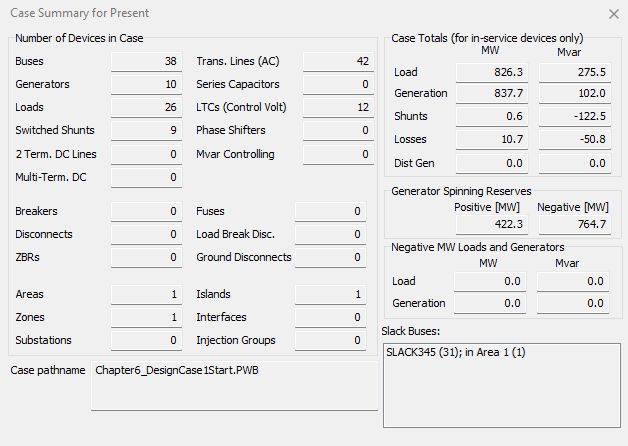
\includegraphics[width=1\linewidth]{figures/case_summary_existing}
	\caption{Case summary for existing system}
	\label{fig:casesummaryexisting}
\end{figure}
\subsection{Contingency Analysis}
PowerWorld's contingency analysis examines conditions when each element of the power system is taken offline. It reveals vulnerability in the 69 kV network in three contingency violations. Specifically, loss of either the PINE138 transformer or the PINE69-APPLE69 line results in overload, with the OAK69-BUCKEYE69 line experiencing loading up to 110.8\% of its thermal limit. These violations suggest that the existing infrastructure is approaching its capacity limits. 

These results are summarized in Table \ref{tab:violations}. A zoomed-in view of the affected areas of the power system is shown in Figure \ref{fig:baseviolations}.
\begin{table}[htbp]
	\caption{Line violations in contingency analysis}
	\begin{center}
		\begin{tabular}{|l|c|c|c|}
			\hline
			\textbf{Contingency} & \textbf{Flow(A)} & \textbf{Limit(A)} & \textbf{\%} \\
			\hline
			\textit{PINE138-PINE69 Xfmr:} & & & \\
			OAK69-BUCKEYE69 & 760.3 & 686.1 & 110.8 \\
			BUCKEYE69-APPLE69 & 454.2 & 418.4 & 108.6 \\
			\hline
			\textit{PINE69-APPLE69 Line:} & & & \\
			OAK69-BUCKEYE69 & 699.2 & 686.1 & 101.9 \\
			\hline
		\end{tabular}
		\label{tab:violations}
	\end{center}
\end{table}
\begin{figure}[tbph]
	\centering
	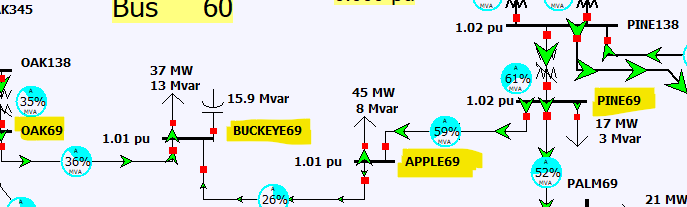
\includegraphics[width=1\linewidth]{figures/base_violations}
	\caption{Existing contingency violations - problem area}
	\label{fig:baseviolations}
\end{figure}
\section{Design}
The design solution must incorporate new transmission infrastructure to connect the 75 MW solar facility at NEWSOLAR while simultaneously addressing existing problems. There must be redundant transmission paths to NEWSOLAR for reliability, meaning at least two separate transmission lines must be constructed. These lines can be either 69 kV or 138 kV, with NEWSOLAR and all existing substations capable of accommodating either voltage level through installation of transformers. The system must maintain all bus voltages between 0.95 and 1.10 per unit and keep all line flows below their thermal limits under both normal operation and any single-contingency (N-1) scenario.

The optimal solution will minimize total cost, calculated as the construction costs minus any savings from reduced system losses over a 5-year period at \$60/MWh. Construction costs include both fixed components (\$1.25M for 138 kV or \$750k for 69 kV lines) and variable costs based on distance and conductor type. If 138 kV is utilized, additional costs include substation upgrades (\$900k per substation) and necessary transformers (\$1.5M for 101 MVA or \$1.8M for 168 MVA). The solution must resolve existing contingency violations, particularly the overloads observed in the OAK69-BUCKEYE69-APPLE69 corridor, while ensuring reliable operation both when the solar plant is at full output and when it is offline.
\subsection{Transmission Line Parameters}
A note on how to input transmission line parameters into PowerWorld is in order. Table A.4 in the text gives resistance in ohms per conductor per mile for 50$^\circ$C at 60Hz as well as series inductance (ohms/mile/conductor for 1 foot spacing) and shunt capacitance (Mohms/mile/conductor for 1 foot spacing). Resistance pulled from Table A.4 can be input directly into the "Calculate Impedances" dialog box in PowerWorld. But for 69kV lines, the three phases are spaced 2m apart and 4m apart for 138kV lines. We need a way to convert the 1-foot spacing parameters appropriately. Assuming equilateral spacing of lines, Equation 4.5.9 in the text suggests a simple way to adjust series inductance. We simply add the following quantity to that given in the table:
\begin{flalign}
	\Delta L_{69} &= 2\pi\cdot60\cdot2\times10^{-7}\left(\ln\frac{D_2}{D_1}\right)\nonumber\\
	&= 2\pi\cdot60\cdot2\times10^{-7}\left(\ln\frac{2}{0.3048}\right) = 0.0001\\
	\Delta L_{138} &= 2\pi\cdot60\cdot2\times10^{-7}\left(\ln\frac{4}{0.3048}\right) = 0.0002.
\end{flalign}

Using Equation 4.9.15 in the text we can develop a multiplication factor to adjust table shunt capacitance values for larger conductor spacing:
\begin{flalign}
	\frac{X_c^\text{new}}{X_c^\text{old}} & = \frac{\ln\left(\frac{D_\text{old}}{r}\right)}{\ln\left(\frac{D_\text{new}}{r}\right)}
\end{flalign}

where $r$ is the conductor's outer radius. Though these are stranded conductors, we treat them as solid since the associated error is small.
\subsection{Candidate Solutions}
With an impractically large set of possible solutions, we started with a couple of simple approaches to integrate the 75 MW solar facility while addressing system reliability concerns. We focused mainly on distance from NEWSOLAR, identifying BUCKEYE and APPLE as the closest stations.

First we attempted to maintain NEWSOLAR at 69kV with new connections to BUCKEYE and APPLE using Condor 900A/107.5MVA conductors. We selected those stations because of their proximity to NEWSOLAR (only 6km each). We upgraded the OAK69-BUCKEYE69 and BUCKEYE69-APPLE69 lines to the highest-rated available 69kV conductor (Condor at 900A). However, contingency analysis revealed voltage violations at OAK138, dropping to 0.939 per unit when the OAK345-OAK138 transformer is opened. This suggests a need for stronger integration with the 138kV network.

Next we installed a 138kV bus at NEWSOLAR with a 138/69kV transformer connecting it to the 69kV bus. Since voltage dropped too low at OAK in the previous design, we connected NEWSOLAR138 to OAK138 using Cardinal 1010A/241.4MVA lines. Since 138kV lines are significantly more expensive than 69kV, we kept the 69kV connection to PINE69. We found a slight overcurrent contingency violation on the OAK69-BUCKEYE69 line when PINE-APPLE is open, so we upgraded it to the 900A Condor lines. With this new configuration there are no contingency violations.

PowerWorld's Case Summary for this configuration shows losses of 10.9MW, a 0.2MW increase from the base scenario. That suggests we should consider upgrading more transmission lines to see if we can achieve enough reduction in loss to offset costs. Contingency analysis showed no violations with this configuration, so we now examine the cost of this approach before considering more upgrades. Table \ref{tab:cost_breakdown_with_losses} shows the breakdown of costs incurred, with a total of \$21,715,600.
\begin{table}[h!]
	\centering
	\begin{tabular}{|l|r|}
		\hline
		\textbf{Modification} & \textbf{Cost (\$)} \\ \hline
		\multicolumn{2}{|l|}{\textbf{Replace OAK-BUCKEYE (69kV Condor)}} \\ 
		\hspace{1em} Fixed Cost & 750,000 \\ 
		\hspace{1em} Variable Cost (\$410,000/km for 8 km) & 3,280,000 \\ 
		\hspace{1em} \textbf{Total} & \textbf{4,030,000} \\ \hline
		\multicolumn{2}{|l|}{\textbf{138-kV Bus/101MVA Transformer}} \\ 
		\hspace{1em} Bus & 900,000 \\ 
		\hspace{1em} Transformer & 1,500,000 \\ 
		\hspace{1em} \textbf{Total} & \textbf{2,400,000} \\ \hline
		\multicolumn{2}{|l|}{\textbf{New Line NEWSOLAR-OAK138 (138kV Cardinal)}} \\ 
		\hspace{1em} Fixed Cost & 1,250,000 \\ 
		\hspace{1em} Variable Cost (\$540,000/km for 13 km) & 7,020,000 \\ 
		\hspace{1em} \textbf{Total} & \textbf{8,270,000} \\ \hline
		\multicolumn{2}{|l|}{\textbf{New Line NEWSOLAR-PINE69 (69kV Condor)}} \\ 
		\hspace{1em} Fixed Cost & 750,000 \\ 
		\hspace{1em} Variable Cost (\$410,000/km for 14 km) & 5,740,000 \\ 
		\hspace{1em} \textbf{Total} & \textbf{6,490,000} \\ \hline
		\textbf{Increased Loss (0.2 MW over 5 years)} & \textbf{525,600} \\ \hline
		\textbf{Grand Total} & \textbf{21,715,600} \\ \hline
	\end{tabular}
	\vspace{0.5em}
	\caption{Cost Breakdown of Option 2}
	\label{tab:cost_breakdown_with_losses}
\end{table}

The massive expense of replacing lines seen in Table \ref{tab:cost_breakdown_with_losses} suggests that loss reduction will not pay for more line upgrades. Next we examine whether there is a better way to connect NEWSOLAR to the grid, perhaps with closer stations.
\section{Conclusion}
Summary of key findings and recommendations
	
\begin{thebibliography}{00}
	\bibitem{b1} PowerWorld Corporation, "PowerWorld Simulator Manual," 2024.
	\bibitem{b2} IEEE Standard 1547-2018, "IEEE Standard for Interconnection and Interoperability of Distributed Energy Resources with Associated Electric Power Systems Interfaces."
\end{thebibliography}

\end{document}